\chapter{Extra information on chapter 3}\label{app:chp3}
\begin{figure}[H]
    \centering
    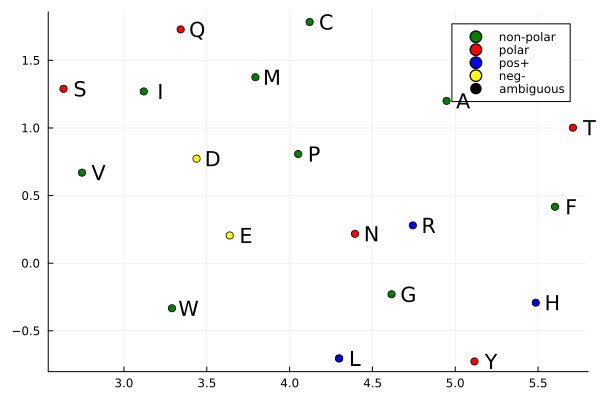
\includegraphics[scale = 0.5]{ur4tr_emb}
    \caption{Scatter plot of a two-dimensional UMAP projection of the average amino acid HDVs with neighborhood-information of $k = 4$ encoded, trained on the human reference proteome. The amino acids are annotated and colored based on their chemical property of polarity. These were made starting from random hyperdimensional vectors.}
    \label{fig:AAtr4ru}
\end{figure}
\begin{figure}[H]
    \centering
    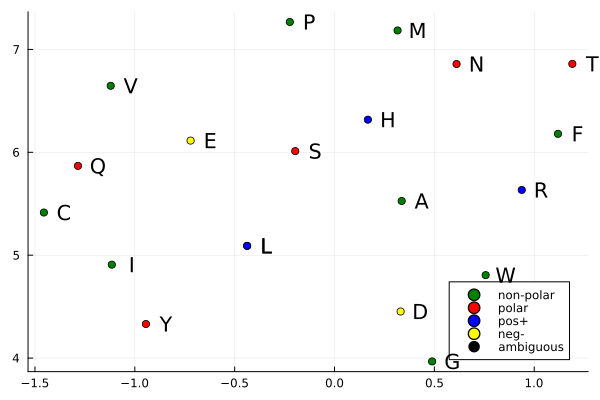
\includegraphics[scale = 0.5]{ur50tr_emb}
    \caption{Scatter plot of a two-dimensional UMAP projection of the average amino acid HDVs with neighborhood-information of $k = 50$ encoded, trained on the human reference proteome. The amino acids are annotated and colored based on their chemical property of polarity. These were made starting from random hyperdimensional vectors.}
    \label{fig:AAtr50ru}
\end{figure}
\begin{figure}[H]
    \centering
    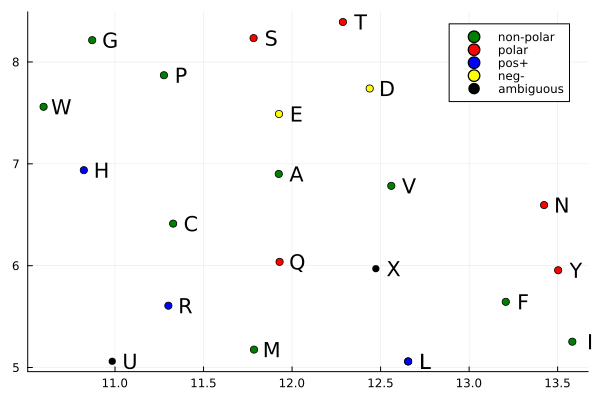
\includegraphics[scale = 0.5]{u4tr_emb}
    \caption{Scatter plot of a two-dimensional UMAP projection of the average amino acid HDVs with neighborhood-information of $k = 4$ encoded, trained on the human reference proteome. The amino acids are annotated and colored based on their chemical property of polarity. These were made starting from extended ESM embeddings.}
    \label{fig:AAtr4u}
\end{figure}
\begin{figure}[H]
    \centering
    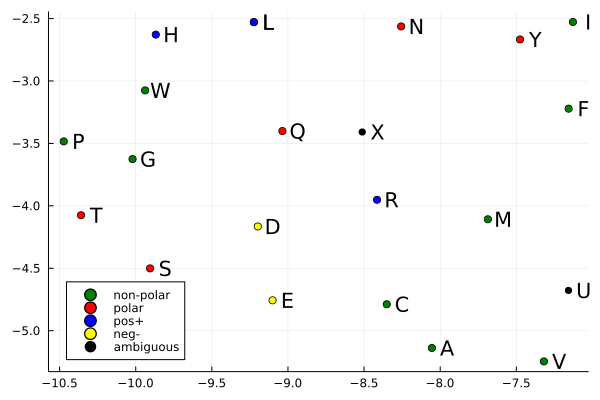
\includegraphics[scale = 0.5]{u50tr_emb}
    \caption{Scatter plot of a two-dimensional UMAP projection of the average amino acid HDVs with neighborhood-information of $k = 50$ encoded, trained on the human reference proteome. The amino acids are annotated and colored based on their chemical property of polarity. These were made starting from extended ESM embeddings.}
    \label{fig:AAtr50u}
\end{figure}